\documentclass{thomasClass}
\usepackage[utf8]{inputenc}

\title{\textbf{Required Practical 11}
\\Production of a dilation series of a glucose solution and use of colorimetric techniques to produce a calibration curve with which to identify the concentration of glucose in an unknown 'urine sample'
}
\author{Thomas Boxall}
\date{January 2022}

\begin{document}

\maketitle

\section{Method}
\begin{enumerate}
    \item Make the serial dilution of glucose and distilled water
    \begin{enumerate}
        \item Label 6 test tubes 0 to 10 mmol dm$^{-3}$ as shown in the table below
        \item Dilute the glucose standard (10 mmol dm$^{-3}$) with water in the labelled test tubes as shown in the table below.
    \end{enumerate}
    \begin{table}[H]
    \centering
    \begin{tabularx}{0.625\textwidth}{l|llllll}
    Conc. of solution / mmol dm$^{-3}$ & 0.0 & 2.0 & 4.0 & 6.0 & 8.0 & 10.0 \\
    \hline
    Vol. of water / $cm^3$ & 2.0 & 1.6 & 1.2 & 0.8 & 0.4 & 0.0 \\
    Vol of glucose standard / $cm^3$  & 0.0 & 0.4 & 0.8 & 1.2 & 1.6 & 2.0
    \end{tabularx}
    \end{table}
    \item Add $2cm^3$ of Benedict's quantitative reagent. Mix well
    \item Heat at 85-90\textdegree C for 4 minutes
    \item Remove from the water bath and allow to cool for 5 to 10 minutes
    \item Pipette most of the supernatant into cuvettes, avoiding the precipitate
    \item Use a colorimeter to measure the absorbance, using 680nm wavelength.
\end{enumerate}

\section{Data tables}
\subsection{Calibration Curve Results}
\begin{table}[H]
\begin{tabularx}{0.5\textwidth}{l|l}
Glucose Concentration & \% Absorbance (a.u) \\
\hline
0.0 & 0.57 \\
2.0 & 0.66 \\
4.0 & 0.73 \\
6.0 & 0.63 \\
8.0 & 0.39 \\
10.0 & 0.96
\end{tabularx}
\end{table}
\subsection{Urine Sample results}
\begin{table}[H]
\begin{tabularx}{0.6\textwidth}{lll}
Sample & \% Absorbance & Estimated Glucose Concentration \\
\hline
Jo & 0.72 &  \\
Christa & 0.56 &  \\
Harjit & 0.97 & 
\end{tabularx}
\end{table}

\section{Graph}
\begin{figure}[H]
    \centering
    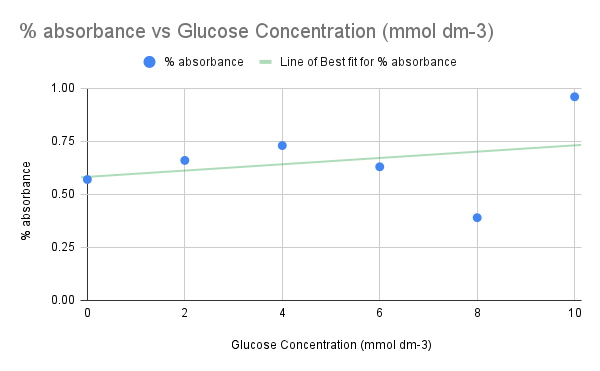
\includegraphics[width=0.8\textwidth]{RPA11-GRAPH.png}

\end{figure}

\section{Evaluating Results}
These results are generally erroneous. For a calibration curve, you would expect the result to plot on a straight line. This concludes that the points at 0.0, 2.0 and 10.0 can be discounted as anomalies.
Due to the anomalous results, it is unscientific to draw the results for the three samples. I would need to repeat the experiment again to be able to draw results.
\end{document}
